\section{Primjer primjene na stvarnim podacima}
\label{pal:sec:primjenanastvarnim}

Iako dublja analiza stvarnih DNA nizova u odnosu na broj palindroma
nije u području ovog doktorskog rada, svejedno će se u ovom potpoglavlju prezentirati
kratka analiza određenog DNA niza kao primjer primjene na stvarnim
podacima. 

Poznata je činjenica da frekvencije nukleobaza variraju
unutar DNA niza 
(\textcite{louie_nucleotide_2003} te \textcite{mrazek_strand_1998}).
Ovo je svojstvo
ilustrirano na slici \ref{pal:fig:AT_freq} za niz
{\glqq}Homo sapiens chromosome 1 genomic contig NT\_077912\_1''
\cite{ncbi_database_homosapiens}
duljine $153\, 649$.
Niz je podijeljen na blokove jednake duljine od
2000 znakova (parova) te su zbrojene frekvencije
komplementarnih baza $A$ i $T$.
Bitno je napomenuti da je duljina blokova odabrana proizvoljno
i ne mora nužno reprezentirati smislenu razdiobu na regije.
No, ukoliko se posjeduje ekspertno znanje o nizu nad kojim
se vrši istraživanje, blokove treba prilagoditi tom znanju.
Ekspertno je znanje od velike važnosti za analizu budući
da se kodirajuće i nekodirajuće regije uglavnom sastoje
od različitih distribucija baza 
(\textcite{roy_identification_2009}).

\begin{figure}
\centering
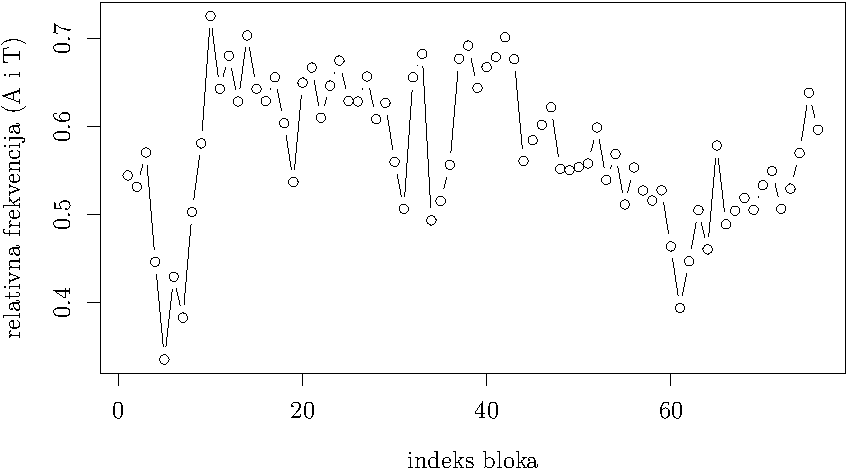
\includegraphics[scale = 1]{poglavlja/palindromi/slike/ATfreq_kromosom_1_blokovi_duljine_2000.pdf}
\caption{Zbrojene frekvencije od $A$ i $T$ po blokovima duljine 2000 za niz
{\glqq}Homo sapiens chromosome 1 genomic contig NT\_077912\_1''
\cite{ncbi_database_homosapiens}}
\label{pal:fig:AT_freq}
\end{figure}

\noindent  
Broj palindroma različitih duljina određen je po blokovima
te je rezultat o asimptotskoj normalnoj distribuciji
(pretpostavljajući da su blokovi tipa T1)
primijenjen pri izračunu vjerojatnosti dobivanja
broja palindroma minimalno velikog kao uočeni
($p$-vrijednosti ukoliko $\frac{N_n-\hat{\mu}_n}{\sqrt{n}}$
smatramo testnom statistikom). Rezultati za
palindrome duljina $6$ i $8$ prezentirani su u tablici
\ref{pal:tab:rezultatinahomosapiensu}. 

\begin{table}[htbp] 
\caption{Duljina niza $n=153\, 649$; za duljinu palindroma $m=6$
	bilo je 2464 palindroma dok je za duljinu palindroma $m=8$
	bilo 694 palindroma.}
\label{pal:tab:rezultatinahomosapiensu}
\centering
\begin{tabular}{ccccccc}
\hline
\multicolumn{1}{c}{} & \multicolumn{3}{c}{$m=6$} & \multicolumn{3}{c}{$m=8$} \\
\cmidrule(lr{0.75em}){2-4} \cmidrule(lr{0.75em}){5-7}
duljina blokova & $\frac{N_n-\hat{\mu}_n}{\sqrt{n}}$ & $\hat{\sigma}^2$ & p-vrijednost
& $\frac{N_n-\hat{\mu}_n}{\sqrt{n}}$ & $\hat{\sigma}^2$ & p-vrijednost \\
\hline
400 & -0.39555 & 0.01783 & 0.00153 & 0.0347 & 0.00458 & 0.3038\\ 
700 & -0.41628 & 0.017767 & 0.00089 & 0.0319 & 0.00456 & 0.3181\\ 
1000 & -0.42335  & 0.01772 & 0.00073 & 0.0322 & 0.00455 & 0.3162\\ 
1300 & -0.44870 & 0.01775 & 0.00037  & 0.0234 & 0.00457 & 0.3646\\ 
2000 & -0.45280 & 0.01770 & 0.00033  & 0.0236 & 0.00456 & 0.3633\\ 
n (n.j.d.) & -0.18075 & 0.01654 & 0.07995 & 0.12424  & 0.00422 & 0.02798\\ 
\hline 
\end{tabular} 
\end{table}

\noindent
Zanimljivo je primijetiti nepodudaranje modela s blokovima
s modelom u kojem pretpostavljamo nezavisnost i jednaku
distribuiranost. Za duljinu palindroma $m=6$ broj 
palindroma proglasili bi iznimnim, uz razinu značajnosti
od 5\%, za modele s blokovima dok istu vrijednost ne bi
proglasili iznimnom po n.j.d. modelu.
Obrnut slučaj možemo primijetiti kod palindroma duljine $m=8$
jer modeli s blokovima ne ukazuju na iznimnost za razliku od
n.j.d. modela.

Ovaj primjer tako pokazuje da bi korištenje n.j.d. modela moglo
dovesti do krivog tumačenja. Razlog leži u regijama s visokim
očekivanim brojem palindroma (zbog visokog postotka
komplementarnih baza) pa korištenjem n.j.d. modela
gubimo tu informaciju budući da usrednjavamo frekvencije.
Slobodno govoreći, model s blokovima je sposoban prepoznati
razlike među regijama dok n.j.d. model to isto nije sposoban
prepoznati. Stoga, n.j.d. model treba koristiti s oprezom.

Također, zanimljivo je primijetiti da se promjenom veličine
blokova p-vrijednosti ne mijenjaju znatno.

